\chapter{Validation croisée des simulations}

\section{Convertisseur CC-CC 4 quadrants formé de 2 convertisseurs 3 niveaux NPC}

\begin{figure}[htb]
\centering
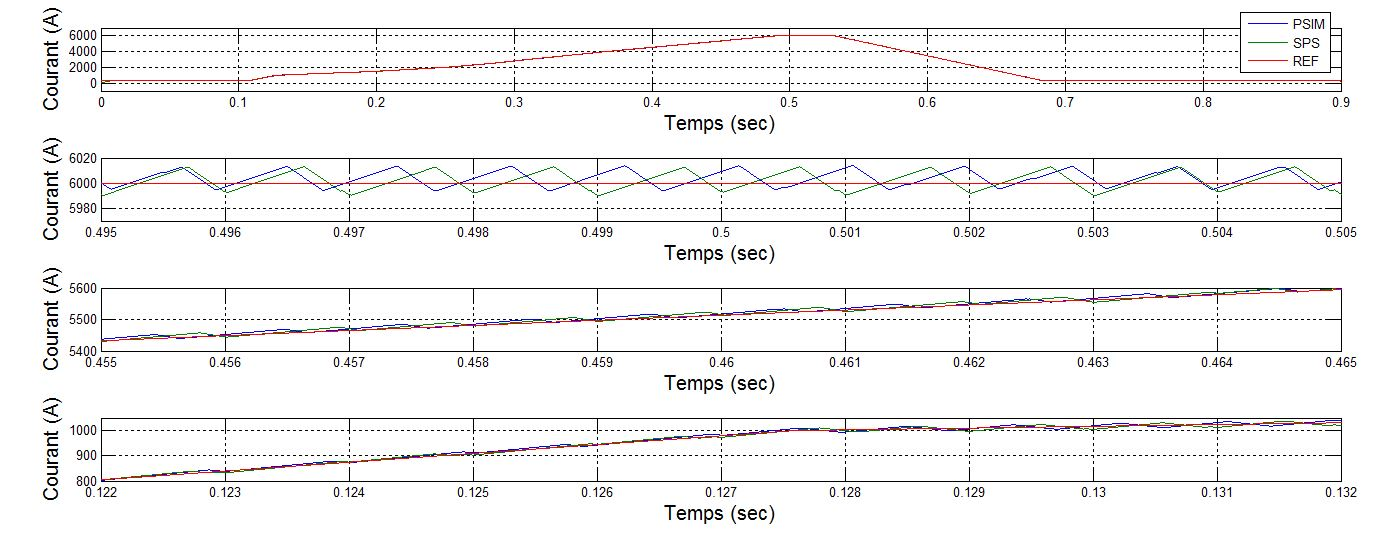
\includegraphics[scale=0.5]{fig/DCPDCN/DCPCourantCharge1u.jpg}
\caption{Courant traversant la charge sur PSIM et SPS pour un pas de calcul de 1$\mu$s pour le DCP/DCN}
\label{DC_ch_cou_1}
\end{figure}

\begin{figure}[htb]
\centering
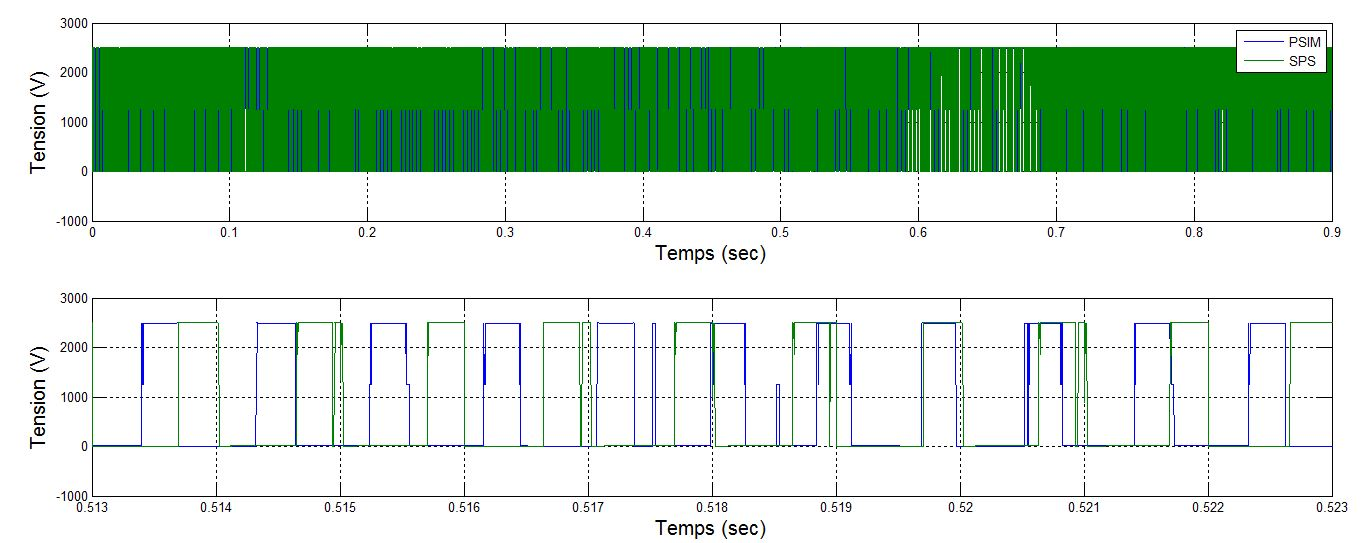
\includegraphics[scale=0.5]{fig/DCPDCN/DCPTensionIGBT1u.jpg}
\caption{Tension aux bornes d'un IGBT sur PSIM et SPS pour un pas de calcul de 1$\mu$s pour le DCP/DCN}
\label{DC_IG_ten_1}
\end{figure}

\section{AFE 3 niveaux NPC avec contrôle par MLI}

\begin{figure}[htb]
\centering
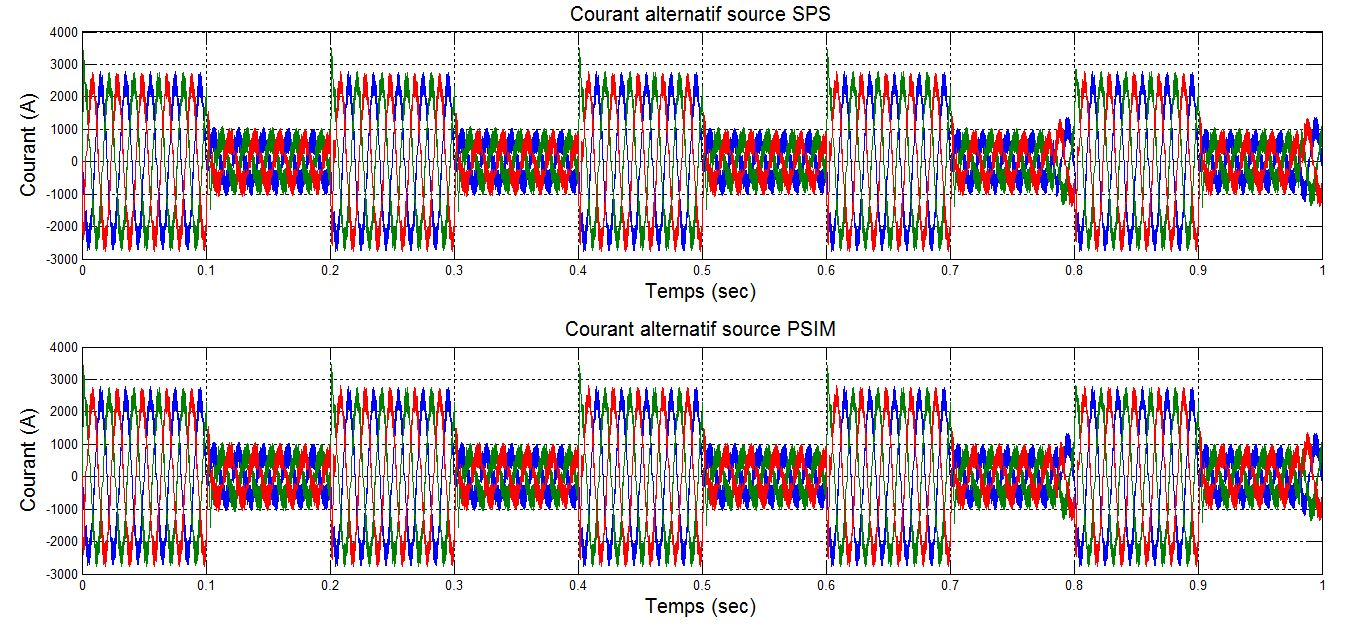
\includegraphics[scale=0.5]{fig/coual_afe.jpg}
\caption{Le courant d'entré à 1$\mu$s pour l'AFE sur charge RC}
\label{AF_RC_cou}
\end{figure}




\begin{figure}[htb]
\centering
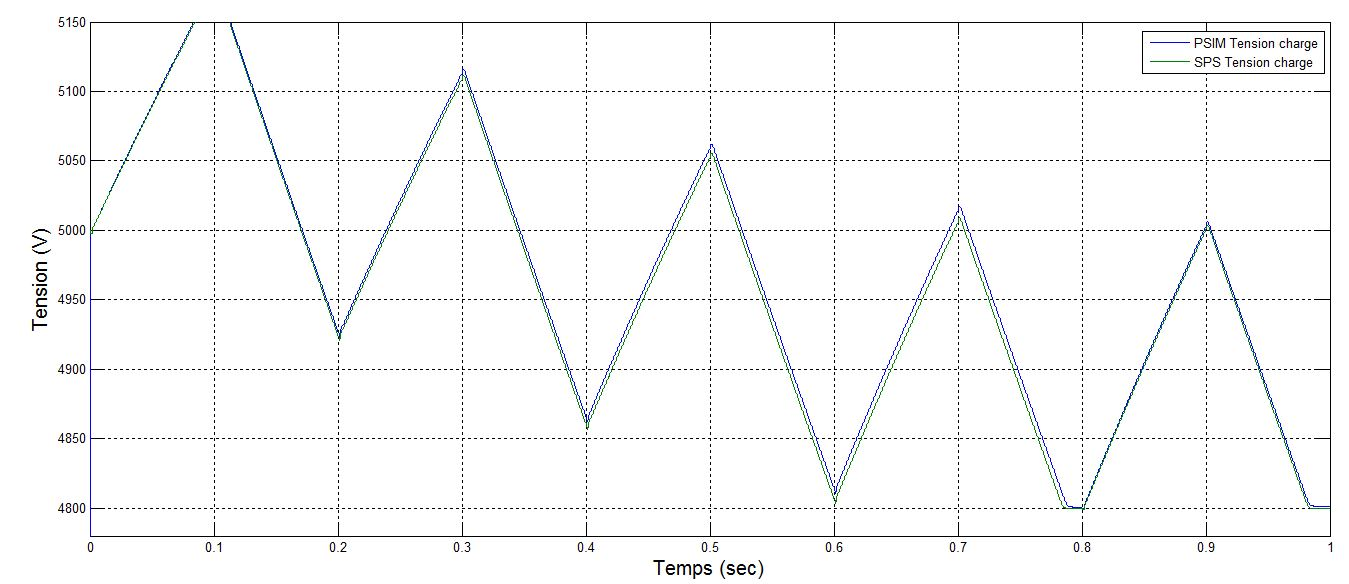
\includegraphics[scale=0.5]{fig/ten_afe.jpg}
\caption{La tension à la charge à 1$\mu$s pour l'AFE sur charge RC}
\label{AF_RC_ten}
\end{figure}



\begin{figure}[htb]
\centering
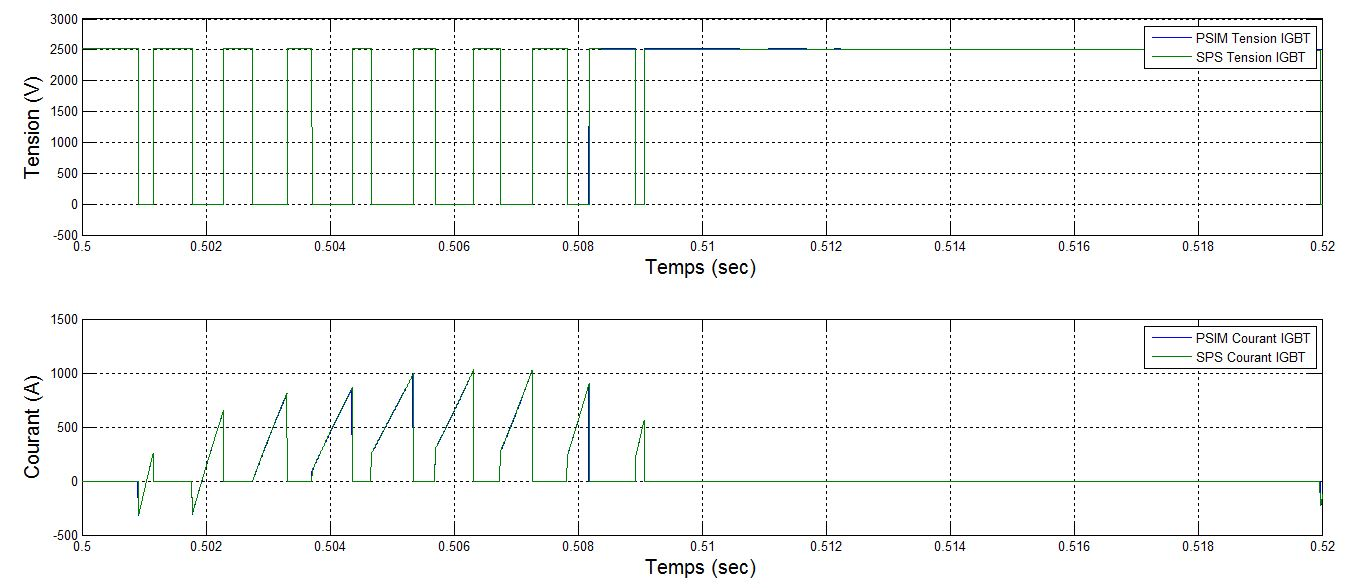
\includegraphics[scale=0.5]{fig/com_afe.jpg}
\caption{La tension et le courant au bornes d'un IGBT à 1$\mu$s pour l'AFE sur charge RC}
\label{AF_RC_igbt}
\end{figure}

\section{AFE 3 niveaux NPC avec contrôle par MLI avec convertisseur CC-CC formé de 2 cellules NPC 3 niveaux}

\begin{figure}[htb]
\centering
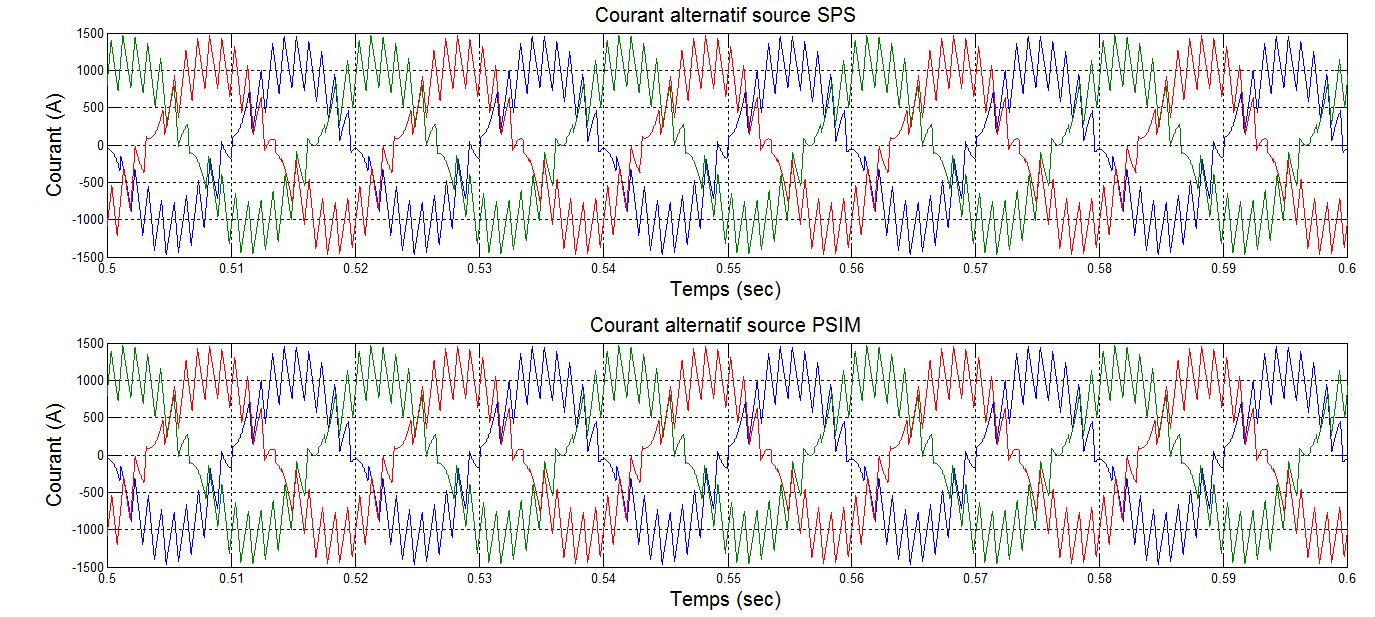
\includegraphics[scale=0.5]{fig/DCP_AFE/1u/cour_al.jpg}
\caption{Le courant d'entrée de l'AFE pour un pas de calcul de 1$\mu$s}
\label{AF_DC_cou1}
\end{figure}


\begin{figure}[htb]
\centering
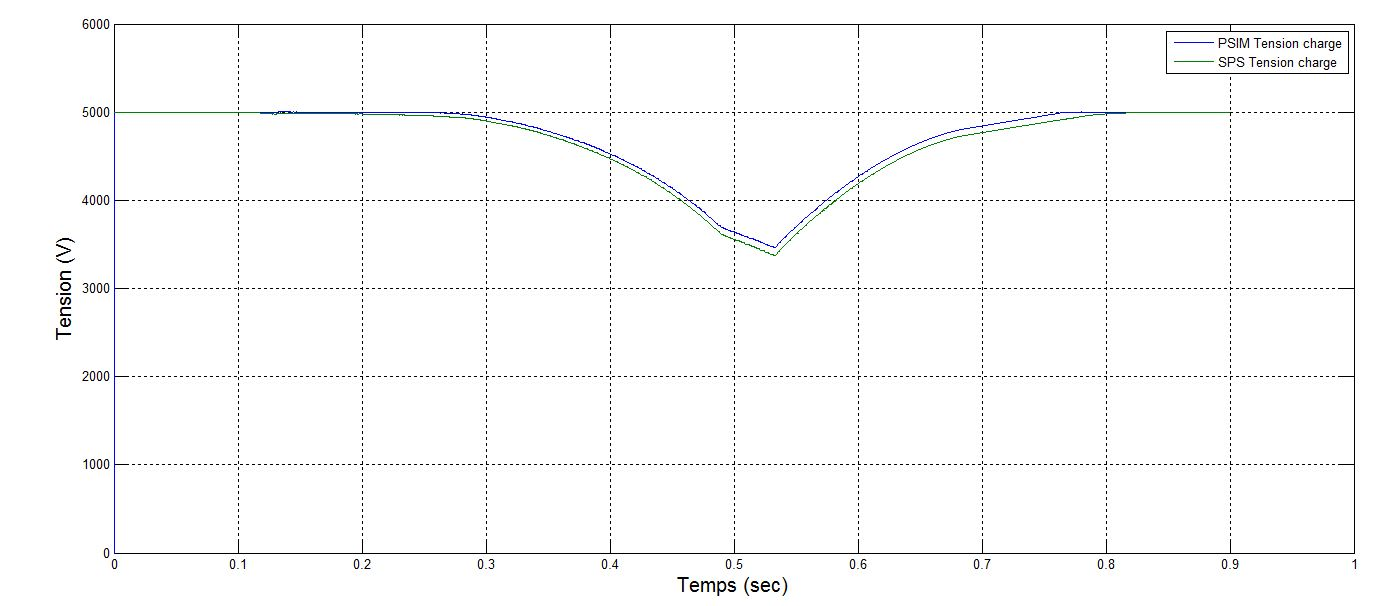
\includegraphics[scale=0.5]{fig/DCP_AFE/1u/ten_bus.jpg}
\caption{La tension du bus CC pour un pas de calcul de 1$\mu$s}
\label{AF_DC_vch1}
\end{figure}

\begin{figure}[htb]
\centering
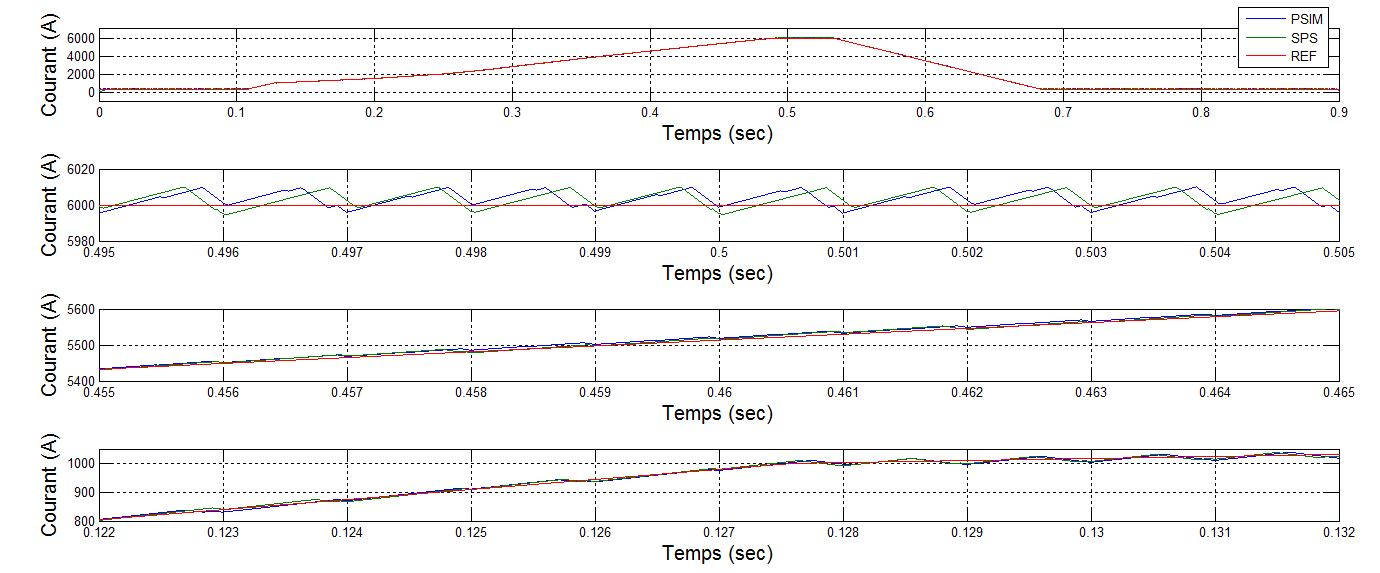
\includegraphics[scale=0.5]{fig/DCP_AFE/1u/cour_ch.jpg}
\caption{Le courant aux bornes des électroaimants pour un pas de calcul de 1$\mu$s}
\label{AF_DC_CHA1}
\end{figure}

\begin{figure}[htb]
\centering
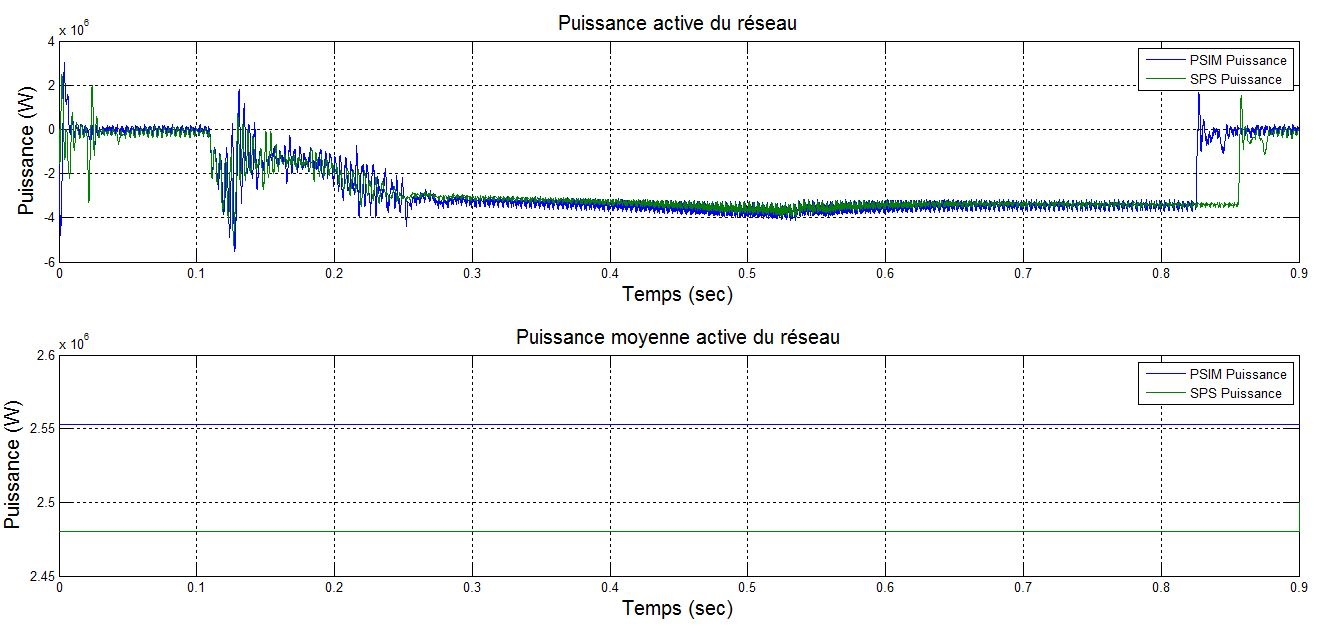
\includegraphics[scale=0.5]{fig/DCP_AFE/1u/PUI.jpg}
\caption{La puissance délivrée par le réseau alternatif pour un pas de calcul de 1$\mu$s}
\label{AF_DC_CHA1}
\end{figure}